%% bare_adv.tex
%% V1.3
%% 2007/01/11
%% by Michael Shell
%% See: 
%% http://www.michaelshell.org/
%% for current contact information.
%%
%% This is a skeleton file demonstrating the advanced use of IEEEtran.cls
%% (requires IEEEtran.cls version 1.7 or later) with an IEEE Computer
%% Society journal paper.
%%
%% Support sites:
%% http://www.michaelshell.org/tex/ieeetran/
%% http://www.ctan.org/tex-archive/macros/latex/contrib/IEEEtran/
%% and
%% http://www.ieee.org/

%%*************************************************************************
%% Legal Notice:
%% This code is offered as-is without any warranty either expressed or
%% implied; without even the implied warranty of MERCHANTABILITY or
%% FITNESS FOR A PARTICULAR PURPOSE! 
%% User assumes all risk.
%% In no event shall IEEE or any contributor to this code be liable for
%% any damages or losses, including, but not limited to, incidental,
%% consequential, or any other damages, resulting from the use or misuse
%% of any information contained here.
%%
%% All comments are the opinions of their respective authors and are not
%% necessarily endorsed by the IEEE.
%%
%% This work is distributed under the LaTeX Project Public License (LPPL)
%% ( http://www.latex-project.org/ ) version 1.3, and may be freely used,
%% distributed and modified. A copy of the LPPL, version 1.3, is included
%% in the base LaTeX documentation of all distributions of LaTeX released
%% 2003/12/01 or later.
%% Retain all contribution notices and credits.
%% ** Modified files should be clearly indicated as such, including  **
%% ** renaming them and changing author support contact information. **
%%
%% File list of work: IEEEtran.cls, IEEEtran_HOWTO.pdf, bare_adv.tex,
%%                    bare_conf.tex, bare_jrnl.tex, bare_jrnl_compsoc.tex
%%*************************************************************************

% *** Authors should verify (and, if needed, correct) their LaTeX system  ***
% *** with the testflow diagnostic prior to trusting their LaTeX platform ***
% *** with production work. IEEE's font choices can trigger bugs that do  ***
% *** not appear when using other class files.                            ***
% The testflow support page is at:
% http://www.michaelshell.org/tex/testflow/



% IEEEtran V1.7 and later provides for these CLASSINPUT macros to allow the
% user to reprogram some IEEEtran.cls defaults if needed. These settings
% override the internal defaults of IEEEtran.cls regardless of which class
% options are used. Do not use these unless you have good reason to do so as
% they can result in nonIEEE compliant documents. User beware. ;)
%
%\newcommand{\CLASSINPUTbaselinestretch}{1.0} % baselinestretch
%\newcommand{\CLASSINPUTinnersidemargin}{1in} % inner side margin
%\newcommand{\CLASSINPUToutersidemargin}{1in} % outer side margin
%\newcommand{\CLASSINPUTtoptextmargin}{1in}   % top text margin
%\newcommand{\CLASSINPUTbottomtextmargin}{1in}% bottom text margin



% Note that the a4paper option is mainly intended so that authors in
% countries using A4 can easily print to A4 and see how their papers will
% look in print - the typesetting of the document will not typically be
% affected with changes in paper size (but the bottom and side margins will).
% Use the testflow package mentioned above to verify correct handling of
% both paper sizes by the user's LaTeX system.
%
% Also note that the "draftcls" or "draftclsnofoot", not "draft", option
% should be used if it is desired that the figures are to be displayed in
% draft mode.
%
\documentclass[12pt,journal,compsoc]{IEEEtran}
% The Computer Society requires 12pt.
% If IEEEtran.cls has not been installed into the LaTeX system files,
% manually specify the path to it like:
% \documentclass[10pt,journal,compsoc]{../sty/IEEEtran}

\usepackage{lipsum} % for dummy text only

% For Computer Society journals, IEEEtran defaults to the use of 
% Palatino/Palladio as is done in IEEE Computer Society journals.
% To go back to Times Roman, you can use this code:
%\renewcommand{\rmdefault}{ptm}\selectfont





% Some very useful LaTeX packages include:
% (uncomment the ones you want to load)



% *** MISC UTILITY PACKAGES ***
%
%\usepackage{ifpdf}
% Heiko Oberdiek's ifpdf.sty is very useful if you need conditional
% compilation based on whether the output is pdf or dvi.
% usage:
% \ifpdf
%   % pdf code
% \else
%   % dvi code
% \fi
% The latest version of ifpdf.sty can be obtained from:
% http://www.ctan.org/tex-archive/macros/latex/contrib/oberdiek/
% Also, note that IEEEtran.cls V1.7 and later provides a builtin
% \ifCLASSINFOpdf conditional that works the same way.
% When switching from latex to pdflatex and vice-versa, the compiler may
% have to be run twice to clear warning/error messages.






% *** CITATION PACKAGES ***
%
\ifCLASSOPTIONcompsoc
  % IEEE Computer Society needs nocompress option
  % requires cite.sty v4.0 or later (November 2003)
  \usepackage[nocompress]{cite}
\else
  % normal IEEE
  % \usepackage{cite}
\fi
% cite.sty was written by Donald Arseneau
% V1.6 and later of IEEEtran pre-defines the format of the cite.sty package
% \cite{} output to follow that of IEEE. Loading the cite package will
% result in citation numbers being automatically sorted and properly
% "compressed/ranged". e.g., [1], [9], [2], [7], [5], [6] without using
% cite.sty will become [1], [2], [5]--[7], [9] using cite.sty. cite.sty's
% \cite will automatically add leading space, if needed. Use cite.sty's
% noadjust option (cite.sty V3.8 and later) if you want to turn this off.
% cite.sty is already installed on most LaTeX systems. Be sure and use
% version 4.0 (2003-05-27) and later if using hyperref.sty. cite.sty does
% not currently provide for hyperlinked citations.
% The latest version can be obtained at:
% http://www.ctan.org/tex-archive/macros/latex/contrib/cite/
% The documentation is contained in the cite.sty file itself.
%
% Note that some packages require special options to format as the Computer
% Society requires. In particular, Computer Society  papers do not use
% compressed citation ranges as is done in typical IEEE papers
% (e.g., [1]-[4]). Instead, they list every citation separately in order
% (e.g., [1], [2], [3], [4]). To get the latter we need to load the cite
% package with the nocompress option which is supported by cite.sty v4.0
% and later. Note also the use of a CLASSOPTION conditional provided by
% IEEEtran.cls V1.7 and later.





% *** GRAPHICS RELATED PACKAGES ***
%
\ifCLASSINFOpdf
  % \usepackage[pdftex]{graphicx}
  % declare the path(s) where your graphic files are
  % \graphicspath{{../pdf/}{../jpeg/}}
  % and their extensions so you won't have to specify these with
  % every instance of \includegraphics
  % \DeclareGraphicsExtensions{.pdf,.jpeg,.png}
\else
  % or other class option (dvipsone, dvipdf, if not using dvips). graphicx
  % will default to the driver specified in the system graphics.cfg if no
  % driver is specified.
  % \usepackage[dvips]{graphicx}
  % declare the path(s) where your graphic files are
  % \graphicspath{{../eps/}}
  % and their extensions so you won't have to specify these with
  % every instance of \includegraphics
  % \DeclareGraphicsExtensions{.eps}
\fi
% graphicx was written by David Carlisle and Sebastian Rahtz. It is
% required if you want graphics, photos, etc. graphicx.sty is already
% installed on most LaTeX systems. The latest version and documentation can
% be obtained at: 
% http://www.ctan.org/tex-archive/macros/latex/required/graphics/
% Another good source of documentation is "Using Imported Graphics in
% LaTeX2e" by Keith Reckdahl which can be found as epslatex.ps or
% epslatex.pdf at: http://www.ctan.org/tex-archive/info/
%
% latex, and pdflatex in dvi mode, support graphics in encapsulated
% postscript (.eps) format. pdflatex in pdf mode supports graphics
% in .pdf, .jpeg, .png and .mps (metapost) formats. Users should ensure
% that all non-photo figures use a vector format (.eps, .pdf, .mps) and
% not a bitmapped formats (.jpeg, .png). IEEE frowns on bitmapped formats
% which can result in "jaggedy"/blurry rendering of lines and letters as
% well as large increases in file sizes.
%
% You can find documentation about the pdfTeX application at:
% http://www.tug.org/applications/pdftex



%\usepackage{ps4pdf}
% dvi->ps workflow is required to use such packages as psfrag.sty and
% pstricks.sty. However, Rolf Niepraschk's ps4pdf.sty provides a way to
% apply psfrag/pstricks effects to .eps figures and then get the resultant
% figures in .pdf form. Thus, providing an easier way for migrating from
% .eps to .pdf figures. After ps4pdf.sty loads, if:
% 1. producing .dvi output: the output file will consist ONLY of the
%    figures (or other constructs encased within \PSforPDF commands)
% 2. producing .pdf output: pdflatex will look in the filename-pics.pdf
%    file, where filename is the basename of the tex document, for the
%    graphics (or other constructs encased within \PSforPDF commands).
%    NOTE: If you ever change your figures, you must remember to remake
%    the filename-pics.pdf file.
%
% This way you can do a:
% 
% latex filename
% dvips -Ppdf -o filename-pics.ps filename.dvi
% ps2pdf filename-pics.ps filename-pics.pdf
% 
% to produce a filename-pics.pdf graphics container that contains
% .pdf versions of the graphics with psfrag, pstricks, etc. features.
% Note that you will not typically be able to view the figures in 
% filename-pics.ps because of an offset. However, you will be able to
% view them in filename-pics.pdf. Also, note that when ps4pdf is in effect
% with .dvi output, you may get harmless over/under full box warnings - 
% ignore them. 
% Then, run pdflatex:
% 
% pdflatex filename
% 
% to use pdflatex to make PDF output, automatically using the figures in
% filename-pics.pdf. Alternatively, you could use dvips -i option to
% obtain separate .pdf files for each figure:
%
% dvips -Ppdf -i -E -o fig filename
%
% then convert each figure to pdf via a command such as epstopdf and then
% use pdflatex with these pdf figures and then to dispense with ps4pdf.
%
% Remember to rerun through latex/dvips/ps2pdf if you ever change your
% figures so that filename-pics.pdf gets updated.
% ps4pdf requires David Kastrup's preview-latex and a recent LaTeX system
% (circa 2001 or later). The ps4pdf package and documentation can be
% obtained at: http://www.ctan.org/tex-archive/macros/latex/contrib/ps4pdf/
% The preview-latex package and documentation can be obtained at:
% http://www.ctan.org/tex-archive/macros/latex/contrib/preview/
%
% provide a bogus \PSforPDF, even when not loading pd4pdf. This way we can
% stop loading ps4pdf.sty if we choose to make separate .pdf versions of
% each of our figures.
\providecommand{\PSforPDF}[1]{#1}
% Note that in order for ps4pdf to work, all commands related to psfrag,
% pstricks, etc. must be called within the PSforPDF command. This applies
% even when *loading* via \usepackage psfrag.sty, etc.


%\PSforPDF{\usepackage{psfrag}}
% psfrag.sty was written by Craig Barratt, Michael C. Grant, and
% David Carlisle. It allows you to substitute LaTeX commands for text in
% imported EPS graphic files. In this way, LaTeX symbols can be placed into
% graphics that have been generated by other applications. You must use
% latex->dvips->ps2pdf workflow (not direct pdf output from pdflatex) if
% you wish to use this capability because it works via some PostScript
% tricks. Alternatively, the graphics could be processed as separate files
% via psfrag and dvips, then converted to PDF for inclusion in the main file
% which uses pdflatex. ps4pdf.sty (above) provides a way of doing this all
% at once within the main file.
% Docs are in "The PSfrag System" by Michael C. Grant and David Carlisle.
% There is also some information about using psfrag in "Using Imported
% Graphics in LaTeX2e" by Keith Reckdahl which documents the graphicx
% package (see above). The psfrag package and documentation can be obtained
% at: http://www.ctan.org/tex-archive/macros/latex/contrib/psfrag/
% 
% Note that the current version of psfrag does not "turn itself off" when
% running under pdf output. This will result in a harmless warning
% about a non-PDF \special. However, to silence this, a bogus psfrag
% command can be provided instead of loading psfrag.sty when PDF output
% is being used. Thus, a more complex alternative conditional loading scheme
% can be employed instead of the straightforword way above:
%
%\ifCLASSINFOpdf
% if outputting PDF, do not use or load psfrag.sty as current versions
% output a non-PDF special that generates a harmless, but annoying warning.
% Instead, we provide a bogus \psfrag command that does nothing with
% its arguments. This is a tad tricky because \psfrag can have up to six
% arguments four of which are optional: \psfrag{}[][][][]{}
% Code based on that in psfrag.sty
%\makeatletter
%\def\psfrag{\@ifstar{\@BOGUSpsfraga}{\@BOGUSpsfraga}}
%\def\@BOGUSpsfraga{\begingroup
%   \@makeother\"\@makeother\*\@makeother\!\@makeother\~%
%   \@makeother\:\@makeother\\\@makeother\%\@makeother\#%
%   \@makeother\ \@BOGUSpsfragb}
%\def\@BOGUSpsfragb#1{\endgroup
%                \@ifnextchar [{\@BOGUSpsfragc}%
%                              {\@BOGUSpsfrag}}
%\def\@BOGUSpsfragc[#1]{\@ifnextchar [{\@BOGUSpsfragd}%
%                                     {\@BOGUSpsfrag}}
%\def\@BOGUSpsfragd[#1]{\@ifnextchar [{\@BOGUSpsfrage}%
%                                     {\@BOGUSpsfrag}}
%\def\@BOGUSpsfrage[#1]{\@ifnextchar [{\@BOGUSpsfragf}%
%                                     {\@BOGUSpsfrag}}
%\def\@BOGUSpsfragf[#1]{\@BOGUSpsfrag}
%\def\@BOGUSpsfrag#1{\ignorespaces}
%\makeatother
%\else
% using dvi output, load psfrag, but funnel it through PSforPDF
% as required by ps4pdf.sty
%\PSforPDF{\usepackage{psfrag}}
%\fi





% *** MATH PACKAGES ***
%
%\usepackage[cmex10]{amsmath}
% A popular package from the American Mathematical Society that provides
% many useful and powerful commands for dealing with mathematics. If using
% it, be sure to load this package with the cmex10 option to ensure that
% only type 1 fonts will utilized at all point sizes. Without this option,
% it is possible that some math symbols, particularly those within
% footnotes, will be rendered in bitmap form which will result in a
% document that can not be IEEE Xplore compliant!
%
% Also, note that the amsmath package sets \interdisplaylinepenalty to 10000
% thus preventing page breaks from occurring within multiline equations. Use:
%\interdisplaylinepenalty=2500
% after loading amsmath to restore such page breaks as IEEEtran.cls normally
% does. amsmath.sty is already installed on most LaTeX systems. The latest
% version and documentation can be obtained at:
% http://www.ctan.org/tex-archive/macros/latex/required/amslatex/math/





% *** SPECIALIZED LIST PACKAGES ***
%\usepackage{acronym}
% acronym.sty was written by Tobias Oetiker. This package provides tools for
% managing documents with large numbers of acronyms. (You don't *have* to
% use this package - unless you have a lot of acronyms, you may feel that
% such package management of them is bit of an overkill.)
% Do note that the acronym environment (which lists acronyms) will have a
% problem when used under IEEEtran.cls because acronym.sty relies on the
% description list environment - which IEEEtran.cls has customized for
% producing IEEE style lists. A workaround is to declared the longest
% label width via the IEEEtran.cls \IEEEiedlistdecl global control:
%
% \renewcommand{\IEEEiedlistdecl}{\IEEEsetlabelwidth{SONET}}
% \begin{acronym}
%
% \end{acronym}
% \renewcommand{\IEEEiedlistdecl}{\relax}% remember to reset \IEEEiedlistdecl
%
% instead of using the acronym environment's optional argument.
% The latest version and documentation can be obtained at:
% http://www.ctan.org/tex-archive/macros/latex/contrib/acronym/


%\usepackage{algorithmic}
% algorithmic.sty was written by Peter Williams and Rogerio Brito.
% This package provides an algorithmic environment fo describing algorithms.
% You can use the algorithmic environment in-text or within a figure
% environment to provide for a floating algorithm. Do NOT use the algorithm
% floating environment provided by algorithm.sty (by the same authors) or
% algorithm2e.sty (by Christophe Fiorio) as IEEE does not use dedicated
% algorithm float types and packages that provide these will not provide
% correct IEEE style captions. The latest version and documentation of
% algorithmic.sty can be obtained at:
% http://www.ctan.org/tex-archive/macros/latex/contrib/algorithms/
% There is also a support site at:
% http://algorithms.berlios.de/index.html
% Also of interest may be the (relatively newer and more customizable)
% algorithmicx.sty package by Szasz Janos:
% http://www.ctan.org/tex-archive/macros/latex/contrib/algorithmicx/




% *** ALIGNMENT PACKAGES ***
%
%\usepackage{array}
% Frank Mittelbach's and David Carlisle's array.sty patches and improves
% the standard LaTeX2e array and tabular environments to provide better
% appearance and additional user controls. As the default LaTeX2e table
% generation code is lacking to the point of almost being broken with
% respect to the quality of the end results, all users are strongly
% advised to use an enhanced (at the very least that provided by array.sty)
% set of table tools. array.sty is already installed on most systems. The
% latest version and documentation can be obtained at:
% http://www.ctan.org/tex-archive/macros/latex/required/tools/


%\usepackage{mdwmath}
%\usepackage{mdwtab}
% Also highly recommended is Mark Wooding's extremely powerful MDW tools,
% especially mdwmath.sty and mdwtab.sty which are used to format equations
% and tables, respectively. The MDWtools set is already installed on most
% LaTeX systems. The lastest version and documentation is available at:
% http://www.ctan.org/tex-archive/macros/latex/contrib/mdwtools/


% IEEEtran contains the IEEEeqnarray family of commands that can be used to
% generate multiline equations as well as matrices, tables, etc., of high
% quality.


%\usepackage{eqparbox}
% Also of notable interest is Scott Pakin's eqparbox package for creating
% (automatically sized) equal width boxes - aka "natural width parboxes".
% Available at:
% http://www.ctan.org/tex-archive/macros/latex/contrib/eqparbox/





% *** SUBFIGURE PACKAGES ***
%\ifCLASSOPTIONcompsoc
%\usepackage[tight,normalsize,sf,SF]{subfigure}
%\else
%\usepackage[tight,footnotesize]{subfigure}
%\fi
% subfigure.sty was written by Steven Douglas Cochran. This package makes it
% easy to put subfigures in your figures. e.g., "Figure 1a and 1b". For IEEE
% work, it is a good idea to load it with the tight package option to reduce
% the amount of white space around the subfigures. Computer Society papers
% use a larger font and \sffamily font for their captions, hence the
% additional options needed under compsoc mode. subfigure.sty is already
% installed on most LaTeX systems. The latest version and documentation can
% be obtained at:
% http://www.ctan.org/tex-archive/obsolete/macros/latex/contrib/subfigure/
% subfigure.sty has been superceeded by subfig.sty.


%\ifCLASSOPTIONcompsoc
%  \usepackage[caption=false]{caption}
%  \usepackage[font=normalsize,labelfont=sf,textfont=sf]{subfig}
%\else
%  \usepackage[caption=false]{caption}
%  \usepackage[font=footnotesize]{subfig}
%\fi
% subfig.sty, also written by Steven Douglas Cochran, is the modern
% replacement for subfigure.sty. However, subfig.sty requires and
% automatically loads Axel Sommerfeldt's caption.sty which will override
% IEEEtran.cls handling of captions and this will result in nonIEEE style
% figure/table captions. To prevent this problem, be sure and preload
% caption.sty with its "caption=false" package option. This is will preserve
% IEEEtran.cls handing of captions. Version 1.3 (2005/06/28) and later 
% (recommended due to many improvements over 1.2) of subfig.sty supports
% the caption=false option directly:
%\ifCLASSOPTIONcompsoc
%  \usepackage[caption=false,font=normalsize,labelfont=sf,textfont=sf]{subfig}
%\else
%  \usepackage[caption=false,font=footnotesize]{subfig}
%\fi
%
% The latest version and documentation can be obtained at:
% http://www.ctan.org/tex-archive/macros/latex/contrib/subfig/
% The latest version and documentation of caption.sty can be obtained at:
% http://www.ctan.org/tex-archive/macros/latex/contrib/caption/




% *** FLOAT PACKAGES ***
%
%\usepackage{fixltx2e}
% fixltx2e, the successor to the earlier fix2col.sty, was written by
% Frank Mittelbach and David Carlisle. This package corrects a few problems
% in the LaTeX2e kernel, the most notable of which is that in current
% LaTeX2e releases, the ordering of single and double column floats is not
% guaranteed to be preserved. Thus, an unpatched LaTeX2e can allow a
% single column figure to be placed prior to an earlier double column
% figure. The latest version and documentation can be found at:
% http://www.ctan.org/tex-archive/macros/latex/base/


%\usepackage{stfloats}
% stfloats.sty was written by Sigitas Tolusis. This package gives LaTeX2e
% the ability to do double column floats at the bottom of the page as well
% as the top. (e.g., "\begin{figure*}[!b]" is not normally possible in
% LaTeX2e). It also provides a command:
%\fnbelowfloat
% to enable the placement of footnotes below bottom floats (the standard
% LaTeX2e kernel puts them above bottom floats). This is an invasive package
% which rewrites many portions of the LaTeX2e float routines. It may not work
% with other packages that modify the LaTeX2e float routines. The latest
% version and documentation can be obtained at:
% http://www.ctan.org/tex-archive/macros/latex/contrib/sttools/
% Documentation is contained in the stfloats.sty comments as well as in the
% presfull.pdf file. Do not use the stfloats baselinefloat ability as IEEE
% does not allow \baselineskip to stretch. Authors submitting work to the
% IEEE should note that IEEE rarely uses double column equations and
% that authors should try to avoid such use. Do not be tempted to use the
% cuted.sty or midfloat.sty packages (also by Sigitas Tolusis) as IEEE does
% not format its papers in such ways.


%\ifCLASSOPTIONcaptionsoff
%  \usepackage[nomarkers]{endfloat}
% \let\MYoriglatexcaption\caption
% \renewcommand{\caption}[2][\relax]{\MYoriglatexcaption[#2]{#2}}
%\fi
% endfloat.sty was written by James Darrell McCauley and Jeff Goldberg.
% This package may be useful when used in conjunction with IEEEtran.cls'
% captionsoff option. Some IEEE journals/societies require that submissions
% have lists of figures/tables at the end of the paper and that
% figures/tables without any captions are placed on a page by themselves at
% the end of the document. If needed, the draftcls IEEEtran class option or
% \CLASSINPUTbaselinestretch interface can be used to increase the line
% spacing as well. Be sure and use the nomarkers option of endfloat to
% prevent endfloat from "marking" where the figures would have been placed
% in the text. The two hack lines of code above are a slight modification of
% that suggested by in the endfloat docs (section 8.3.1) to ensure that
% the full captions always appear in the list of figures/tables - even if
% the user used the short optional argument of \caption[]{}.
% IEEE papers do not typically make use of \caption[]'s optional argument,
% so this should not be an issue. A similar trick can be used to disable
% captions of packages such as subfig.sty that lack options to turn off
% the subcaptions:
% For subfig.sty:
% \let\MYorigsubfloat\subfloat
% \renewcommand{\subfloat}[2][\relax]{\MYorigsubfloat[]{#2}}
% For subfigure.sty:
% \let\MYorigsubfigure\subfigure
% \renewcommand{\subfigure}[2][\relax]{\MYorigsubfigure[]{#2}}
% However, the above trick will not work if both optional arguments of
% the \subfloat/subfig command are used. Furthermore, there needs to be a
% description of each subfigure *somewhere* and endfloat does not add
% subfigure captions to its list of figures. Thus, the best approach is to
% avoid the use of subfigure captions (many IEEE journals avoid them anyway)
% and instead reference/explain all the subfigures within the main caption.
% The latest version of endfloat.sty and its documentation can obtained at:
% http://www.ctan.org/tex-archive/macros/latex/contrib/endfloat/
%
% The IEEEtran \ifCLASSOPTIONcaptionsoff conditional can also be used
% later in the document, say, to conditionally put the References on a 
% page by themselves.





% *** PDF, URL AND HYPERLINK PACKAGES ***
%
\usepackage{url}
% url.sty was written by Donald Arseneau. It provides better support for
% handling and breaking URLs. url.sty is already installed on most LaTeX
% systems. The latest version can be obtained at:
% http://www.ctan.org/tex-archive/macros/latex/contrib/misc/
% Read the url.sty source comments for usage information. Basically,
% \url{my_url_here}.


% NOTE: PDF thumbnail features are not required in IEEE papers
%       and their use requires extra complexity and work.
%\ifCLASSINFOpdf
%  \usepackage[pdftex]{thumbpdf}
%\else
%  \usepackage[dvips]{thumbpdf}
%\fi
% thumbpdf.sty and its companion Perl utility were written by Heiko Oberdiek.
% It allows the user a way to produce PDF documents that contain fancy
% thumbnail images of each of the pages (which tools like acrobat reader can
% utilize). This is possible even when using dvi->ps->pdf workflow if the
% correct thumbpdf driver options are used. thumbpdf.sty incorporates the
% file containing the PDF thumbnail information (filename.tpm is used with
% dvips, filename.tpt is used with pdftex, where filename is the base name of
% your tex document) into the final ps or pdf output document. An external
% utility, the thumbpdf *Perl script* is needed to make these .tpm or .tpt
% thumbnail files from a .ps or .pdf version of the document (which obviously
% does not yet contain pdf thumbnails). Thus, one does a:
% 
% thumbpdf filename.pdf 
%
% to make a filename.tpt, and:
%
% thumbpdf --mode dvips filename.ps
%
% to make a filename.tpm which will then be loaded into the document by
% thumbpdf.sty the NEXT time the document is compiled (by pdflatex or
% latex->dvips->ps2pdf). Users must be careful to regenerate the .tpt and/or
% .tpm files if the main document changes and then to recompile the
% document to incorporate the revised thumbnails to ensure that thumbnails
% match the actual pages. It is easy to forget to do this!
% 
% Unix systems come with a Perl interpreter. However, MS Windows users
% will usually have to install a Perl interpreter so that the thumbpdf
% script can be run. The Ghostscript PS/PDF interpreter is also required.
% See the thumbpdf docs for details. The latest version and documentation
% can be obtained at.
% http://www.ctan.org/tex-archive/support/thumbpdf/
% Be sure and use only version 3.8 (2005/07/06) or later of thumbpdf as
% earlier versions will not work properly with recent versions of pdfTeX
% (1.20a and later).


% NOTE: PDF hyperlink and bookmark features are not required in IEEE
%       papers and their use requires extra complexity and work.
% *** IF USING HYPERREF BE SURE AND CHANGE THE EXAMPLE PDF ***
% *** TITLE/SUBJECT/AUTHOR/KEYWORDS INFO BELOW!!           ***
\newcommand\MYhyperrefoptions{bookmarks=true,bookmarksnumbered=true,
pdfpagemode={UseOutlines},plainpages=false,pdfpagelabels=true,
colorlinks=true,linkcolor={black},citecolor={black},pagecolor={black},
urlcolor={black},
pdftitle={Test Driven development in Agile Processes - final quality of the system},%<!CHANGE!
pdfsubject={Typesetting},%<!CHANGE!
pdfauthor={Group 6},%<!CHANGE!
pdfkeywords={Computer Society, IEEEtran, journal, LaTeX, paper,
             template}}%<^!CHANGE!
%\ifCLASSINFOpdf
%\usepackage[\MYhyperrefoptions,pdftex]{hyperref}
%\else
%\usepackage[\MYhyperrefoptions,breaklinks=true,dvips]{hyperref}
%\usepackage{breakurl}
%\fi
% One significant drawback of using hyperref under DVI output is that the
% LaTeX compiler cannot break URLs across lines or pages as can be done
% under pdfLaTeX's PDF output via the hyperref pdftex driver. This is
% probably the single most important capability distinction between the
% DVI and PDF output. Perhaps surprisingly, all the other PDF features
% (PDF bookmarks, thumbnails, etc.) can be preserved in
% .tex->.dvi->.ps->.pdf workflow if the respective packages/scripts are
% loaded/invoked with the correct driver options (dvips, etc.). 
% As most IEEE papers use URLs sparingly (mainly in the references), this
% may not be as big an issue as with other publications.
%
% That said, recently Vilar Camara Neto introduced his breakurl.sty
% package which permits hyperref to easily break URLs even in dvi
% mode. Note that breakurl, unlike most other packages, must be loaded
% AFTER hyperref. The latest version of breakurl and its documentation can
% be obtained at:
% http://www.ctan.org/tex-archive/macros/latex/contrib/breakurl/
% breakurl.sty is not for use under pdflatex pdf mode. Versions 1.10 
% (September 23, 2005) and later are recommened to avoid bugs in earlier
% releases.
%
% The advanced features offer by hyperref.sty are not required for IEEE
% submission, so users should weigh these features against the added
% complexity of use. Users who wish to use hyperref *must* ensure that
% their hyperref version is 6.72u or later *and* IEEEtran.cls is version
% 1.6b or later.
% The package options above demonstrate how to enable PDF bookmarks
% (a type of table of contents viewable in Acrobat Reader) as well as
% PDF document information (title, subject, author and keywords) that is
% viewable in Acrobat reader's Document_Properties menu. PDF document
% information is also used extensively to automate the cataloging of PDF
% documents. The above set of options ensures that hyperlinks will not be
% colored in the text and thus will not be visible in the printed page,
% but will be active on "mouse over". USING COLORS OR OTHER HIGHLIGHTING
% OF HYPERLINKS CAN RESULT IN DOCUMENT REJECTION BY THE IEEE, especially if
% these appear on the "printed" page. IF IN DOUBT, ASK THE RELEVANT
% SUBMISSION EDITOR. You may need to add the option hypertexnames=false if
% you used duplicate equation numbers, etc., but this should not be needed
% in normal IEEE work.
% The latest version of hyperref and its documentation can be obtained at:
% http://www.ctan.org/tex-archive/macros/latex/contrib/hyperref/





% *** Do not adjust lengths that control margins, column widths, etc. ***
% *** Do not use packages that alter fonts (such as pslatex).         ***
% There should be no need to do such things with IEEEtran.cls V1.6 and later.
% (Unless specifically asked to do so by the journal or conference you plan
% to submit to, of course. )


% correct bad hyphenation here
\hyphenation{op-tical net-works semi-conduc-tor}

\begin{document}
%
% paper title
% can use linebreaks \\ within to get better formatting as desired
\title{Test Driven Development in Agile Processes - Final quality of the product}
%
%
% author names and IEEE memberships
% note positions of commas and nonbreaking spaces ( ~ ) LaTeX will not break
% a structure at a ~ so this keeps an author's name from being broken across
% two lines.
% use \thanks{} to gain access to the first footnote area
% a separate \thanks must be used for each paragraph as LaTeX2e's \thanks
% was not built to handle multiple paragraphs
%
%
%\IEEEcompsocitemizethanks is a special \thanks that produces the bulleted
% lists the Computer Society journals use for "first footnote" author
% affiliations. Use \IEEEcompsocthanksitem which works much like \item
% for each affiliation group. When not in compsoc mode,
% \IEEEcompsocitemizethanks becomes like \thanks and
% \IEEEcompsocthanksitem becomes a line break with idention. This
% facilitates dual compilation, although admittedly the differences in the
% desired content of \author between the different types of papers makes a
% one-size-fits-all approach a daunting prospect. For instance, compsoc 
% journal papers have the author affiliations above the "Manuscript
% received ..."  text while in non-compsoc journals this is reversed. Sigh.

\author{Carl~Bjerggaard, Johan~Hallberg, Stefan~Johansson, Kristofer~Jacobson, Patrick~Ivarsson% <-this % stops a space
%\IEEEcompsocitemizethanks{\IEEEcompsocthanksitem M. Shell is with the Department
%of Electrical and Computer Engineering, Georgia Institute of Technology, Atlanta,
%GA, 30332.\protect\\
%% note need leading \protect in front of \\ to get a newline within \thanks as
% \\ is fragile and will error, could use \hfil\break instead.
%E-mail: see http://www.michaelshell.org/contact.html
%\IEEEcompsocthanksitem J. Doe and J. Doe are with Anonymous University.}% <-this % stops a space
%\thanks{Manuscript received April 19, 2005; revised January 11}, 2007.
}

% note the % following the last \IEEEmembership and also \thanks - 
% these prevent an unwanted space from occurring between the last author name
% and the end of the author line. i.e., if you had this:
% 
% \author{....lastname \thanks{...} \thanks{...} }
%                     ^------------^------------^----Do not want these spaces!
%
% a space would be appended to the last name and could cause every name on that
% line to be shifted left slightly. This is one of those "LaTeX things". For
% instance, "\textbf{A} \textbf{B}" will typeset as "A B" not "AB". To get
% "AB" then you have to do: "\textbf{A}\textbf{B}"
% \thanks is no different in this regard, so shield the last } of each \thanks
% that ends a line with a % and do not let a space in before the next \thanks.
% Spaces after \IEEEmembership other than the last one are OK (and needed) as
% you are supposed to have spaces between the names. For what it is worth,
% this is a minor point as most people would not even notice if the said evil
% space somehow managed to creep in.



% The paper headers
%\markboth{Journal of \LaTeX\ Class Files,~Vol.~6, No.~1, January~2007}%
%{Shell \MakeLowercase{\textit{et al.}}: Bare Advanced Demo of IEEEtran.cls for Journals}
% The only time the second header will appear is for the odd numbered pages
% after the title page when using the twoside option.
% 
% *** Note that you probably will NOT want to include the author's ***
% *** name in the headers of peer review papers.                   ***
% You can use \ifCLASSOPTIONpeerreview for conditional compilation here if
% you desire.



% The publisher's ID mark at the bottom of the page is less important with
% Computer Society journal papers as those publications place the marks
% outside of the main text columns and, therefore, unlike regular IEEE
% journals, the available text space is not reduced by their presence.
% If you want to put a publisher's ID mark on the page you can do it like
% this:
%\IEEEpubid{0000--0000/00\$00.00~\copyright~2007 IEEE}
% or like this to get the Computer Society new two part style.
%\IEEEpubid{\makebox[\columnwidth]{\hfill 0000--0000/00/\$00.00~\copyright~2007 IEEE}%
%\hspace{\columnsep}\makebox[\columnwidth]{Published by the IEEE Computer Society\hfill}}
% Remember, if you use this you must call \IEEEpubidadjcol in the second
% column for its text to clear the IEEEpubid mark (Computer Society jorunal
% papers don't need this extra clearance.)



% use for special paper notices
%\IEEEspecialpapernotice{(Invited Paper)}



% for Computer Society papers, we must declare the abstract and index terms
% PRIOR to the title within the \IEEEcompsoctitleabstractindextext IEEEtran
% command as these need to go into the title area created by \maketitle.
\IEEEcompsoctitleabstractindextext{%
\begin{abstract}
\label{abstract}
%\boldmath
\lipsum[1]
\end{abstract}
% IEEEtran.cls defaults to using nonbold math in the Abstract.
% This preserves the distinction between vectors and scalars. However,
% if the journal you are submitting to favors bold math in the abstract,
% then you can use LaTeX's standard command \boldmath at the very start
% of the abstract to achieve this. Many IEEE journals frown on math
% in the abstract anyway. In particular, the Computer Society does
% not want either math or citations to appear in the abstract.

% Note that keywords are not normally used for peerreview papers.
\begin{IEEEkeywords}
Keywords 
\end{IEEEkeywords}}


% make the title area
\maketitle


% To allow for easy dual compilation without having to reenter the
% abstract/keywords data, the \IEEEcompsoctitleabstractindextext text will
% not be used in maketitle, but will appear (i.e., to be "transported")
% here as \IEEEdisplaynotcompsoctitleabstractindextext when compsoc mode
% is not selected <OR> if conference mode is selected - because compsoc
% conference papers position the abstract like regular (non-compsoc)
% papers do!
\IEEEdisplaynotcompsoctitleabstractindextext
% \IEEEdisplaynotcompsoctitleabstractindextext has no effect when using
% compsoc under a non-conference mode.


% For peer review papers, you can put extra information on the cover
% page as needed:
% \ifCLASSOPTIONpeerreview
% \begin{center} \bfseries EDICS Category: 3-BBND \end{center}
% \fi
%
% For peerreview papers, this IEEEtran command inserts a page break and
% creates the second title. It will be ignored for other modes.
\IEEEpeerreviewmaketitle

\section{Introduction}
\label{introduction}
%Introduction: introduce the chosen area. The purpose is to give an introduction to the reader who is not
%familiar to the specific area, but knows software engineering and testing generally.

%This section will introduce the reader to the concept of Test Driven Development in Agile Processes and explain how it is performed and how it differs from other software development processes.

This report concerns the area of Test-first Development in Agile Processes and aims to describe and analyse how the final quality of a system is affected by this development method. 

Despite being an old software development method, Test-first Development, also known as Test Driven Development, TDD, has become more and more popular during the last years, inter alia, due to being a central practise of Extreme Programming, XP~\cite{georgeandwilliams}. In Test-Driven development the developers write unit tests for the functionality they are implementing before they write the actual code~\cite{beckTestDriven}. The method is related to the Test-First practices used in XP, ~\cite{beckXP}, but today it is used with other development methods as well~\cite{MSNET}. 

As described by M\"{u}ller and Hagner in~\cite{mullerandhagner}, TDD urges the developers to:
\begin{itemize}
\item	develop programs more capable of accepting changes
\item 	program faster
\item	increase confidence of both developer and customer by seeing all tests pass as well as fail
\item 	reduce defect rates 
\item	understand the program better
\end{itemize}

\noindent Further, M\"{u}ller and Hagner, ~\cite{mullerandhagner}, describes that TDD aims to:
\begin{itemize}
\item 	ensure that programmed features cannot be lost
\item 	force developers to think about and write unit tests 
\item	automate test execution
\item	prevent a program from regressing due to ongoing testing
\item 	provide a test-suite as basis for refactoring
\end{itemize}

\noindent The TDD process is often compared to more traditional Test-last processes, in terms of development time, resultant code quality and understandability~\cite{georgeandwilliams}, or in terms of programming efficiency, resultant code reliability and program understanding~\cite{mullerandhagner}. 

This project will focus on how the quality measure, as mentioned above, is defined and how it differs amongst the different types of software development processes as well as how it is affected by TDD in Agile Processes. 

% The very first letter is a 2 line initial drop letter followed
% by the rest of the first word in caps (small caps for compsoc).
% 
% form to use if the first word consists of a single letter:
% \IEEEPARstart{A}{demo} file is ....
% 
% form to use if you need the single drop letter followed by
% normal text (unknown if ever used by IEEE):
% \IEEEPARstart{A}{}demo file is ....
% 
% Some journals put the first two words in caps:
% \IEEEPARstart{T}{his demo} file is ....
% 
% Here we have the typical use of a "T" for an initial drop letter
% and "HIS" in caps to complete the first word.
%\IEEEPARstart{T}{his} demo file is intended to serve as a ``starter file''
%for IEEE Computer Society journal papers produced under \LaTeX\ using
%IEEEtran.cls version 1.7 and later.
% You must have at least 2 lines in the paragraph with the drop letter
% (should never be an issue)
%I wish you the best of success.

%\hfill mds
% 
%\hfill January 11, 2007
 
\section{Description}
\label{description}
\input{description}

%Description of the chosen area: summary of the chosen area. The purpose is to describe why, how and
%for which purpose the area is used.

In this section quality will be defined in regard to both code quality and product quality. It will also describe why and how Test Driven Development, TDD, improves the quality of a product as well as the purpose of using TDD.

\subsection{Code~Quality} 
\label{quality}

\begin{figure*}
\begin{center}
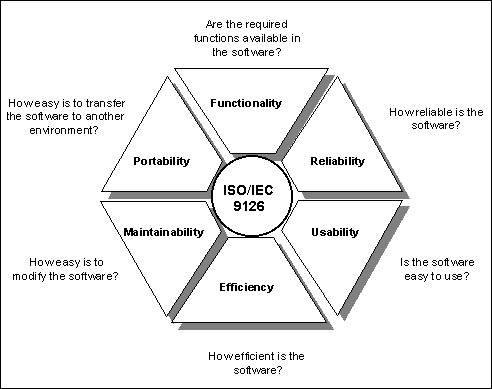
\includegraphics[scale=0.8]{9126ref.png}
\caption{Shows the diffrence between the Test-Last and Test-First workflow}
\end{center}
\end{figure*}

Software is defined from software quality assurance perspective as “combination of computer program (the “code”), procedures, documentation, and data necessary for operating the software the system”~\cite{Galin}. The Software Quality on the other hand defines according to Pressman is “ the degree of conformance to specific functional requirements, specific software quility and Good Software Engineering Practices (GSEP) “~\cite{Pressman}.

This report uses code quality as a term for both “software functional quality” and “Software structural quality” or “Non-functional quality” as Lawrence and Julio~\cite{Chung} describe it where the first one refers more to code per se and the later more to the behavior of the code such as software affection or usability. 

Code quality could be defined and categorized in numerous ways and it has been standardized differently in the past. There is an international standard for product quality ISO-9126 and ISO-25000~\cite{ISO9126}  which defines a basic quality model. This report uses these standard to define Code quality but also the global standard made by “Consortium for IT Software Quality” about business value and costumer satisfaction \url{(http://www.it-cisq.org/cisqwiki/images/8/87/CISQ_2009_Executive_Forums_Report.pdf)} which is based above mentioned standards. 

ISO-9126 is an international standard for product quality and defines six major desirable characteristics which ought to measured in order to guarantee good code quality. Each characteristic is divided into sub-characteristic and further split into attributes which this report do not aim to explain. A good conclusion of the interpretation with 
“Software quality is the degree to which software possesses a desirable combination of attribute (e.g., reliability, interoperability).”~\cite{ISO1061}

The six major characteristics are put forth in the standard are (see fig 1): 
\begin{itemize}
\item Functionality 
\item Reliability
\item Usability
\item Efficiency
\item Maintainability
\item Portability
\end{itemize}	
\subsection{Test Driven Development}
\label{tdd}
With Test-Driven Development (TDD), before writing the actual code, the developer writes unit test cases for the new functionality they are about to implement~\cite{beckTestDriven}. The method is related to the test-first practise used in eXtreme Programming (XP)~\cite{beckXP} but today it’s also used on it’s on together with other development methods~\cite{MSNET}. TDD was used in the 1960’ in the NASA Project Mercury~\cite{NASA} and then rediscovered by Kent Beck (who created XP) in 2003 who claims that it encourages simple design and inspires confidence~\cite{beckXP}. In XP the developers break down things to be implemented into smaller problems, also known as stories. When using TDD with XP, the workflow is according to the scheme below(INSERT BILD REF). After a few test cases are developed the code to make them pass are implemented. Generally the test cases wont even compile before the code is implemented. If the test cases pass, the developer either writes more test cases for the next piece of functionality or moves on to the next story depending on whether the previous story is finished or not. If the test cases fail the developer has to go back and rework the newly implemented code.


By focusing on writing only code necessary to pass tests, designs can be cleaner and clearer than is often achieved by other methods~\cite{beckXP}. When used in XP projects TDD help with the method practice “Simple Design” which basically is keeping the code as simple as possible and only implement functionality that is needed. By doing this the code is easier to work with and it simplifies future integrations. 


When performing TDD developers usually use some sort of test tool. An example of this is JUnit which can be used when developing in Java. JUnit includes a set of assert statements which can be used to verify the output given when unit testing. It also provides Before- and After statements which helps the developer to set up and tear down variables that are needed for several tests. With this functionality, test tools helps the developer manage the vast amount of test cases that are produced.


There are several statements that TDD increasing code quality and productivity~\cite{beckXP}~\cite{erdogmus}. For instance they argue that the test cases are more efficient since the tests have been developed from requirements instead of existing code. However there are others who showed studies that there’s no difference or even a decrease in the overall results~\cite{tddInvest}~\cite{mullerandhagner}. In Section 4 we will try to determine which is more likely based on studies and articles.

\section{Analysis}
\subsection{Benefits of TDD}
\label{benefits}
\subsection{Benefits of TDD} 
The benefits of TDD can be judged by a number of different metrics and circumstances such as the maturity of the developers, test coverage and understandability/maintainability of the code.

Benefits:
\begin{itemize}
\item Gives feedback and supports new design
\item Creates reflection before implementation
\item Improves test coverage
\item Increases productivity by reducing number of defects in the software
\end{itemize}

Gives feedback and support new design
In agile projects the main purpose is to be flexible, ready to change and to have a good collaboration and coordination amongst the developers writing the code. When new code is written and functionality is added to the system the old design is outdated and to avoid patching a system with added features refactoring will be done to integrate the new code and create a good design useful for the system with the current features. 
Since the testcases covers the functionality of the system and not the design the developers can refactor the code and be sure it works as it should. 
In TDD testcases should be written so they test a limited scope of the functionality. This makes it easier for the developer to run regression testing after adding code and makes it easier to pinpoint where in the new code the fault is or which old functionallity the new code conflicts with.

Creates reflection before implementation
Using test-first makes the developer think before he acts. Writing testcases first will force the developer to take into account what the code that will be written shall do and how it will be done[2]. When he then starts to implement the code he has a good idea of how to write it rather than if not using test-first starting implementing code and changing it after coming to new realizations of how to write the code or structure it. The testcases will be written after how the code will work by first analysing the problem and how to best integrate it in the source code and focus on the interface that will be between the new and old code.

Improves test coverage
According to David Scott Janzen[1] more mature developers tend to write more testcases using test-first in contrary to test-last. They also break down the implementation of the functionality to more smaller methods improving the systems understandability, reusability and maintainability. The study[1] made by David Scott Janzen also shows that inexperienced developers tend to do the opposite and write larger methods when using test first, but as they become more experienced they move towards breaking down larger methods into several smaller ones.

Increases productivity by reducing number of defects in the software
The time spent implementing new tasks in a team using TDD is increased because of the additional time it takes to write unit tests. In a study conducted of four projects at Microsoft and IBM[3] using TDD compared to projects not using TDD the teams experienced a 15-35\% loss of productivity. But the products developed had 40-90\% less defects discovered after release compared to equivelent projects not using TDD, which meant that while losing implementation speed TDD acctually increased the overall productivity of the teams.

Referenser:

1. 	An Empirical Evaluation of the Impact of
	Test-Driven Development on Software Quality.

2.	On the Effectiveness of Test-first Approach to Programming
	Erdogmus, Hakan
3.	Realizing quality improvement through test driven
	development: results and experiences of four industrial
	teams





\subsection{Drawbacks of TDD}
\label{drawbacks}
In general TDD has been praised for it's advantages, described in section~\ref{benefits}, but of course it has it's drawbacks.\\

\noindent In this section a drawback will be:
\begin{itemize}
\item an increased production cost, or
\item a decreased code quality, as defined in section~\ref{quality}.
\end{itemize}

According to \textit{\url{http://www.sciencedirect.com/science?_ob=MiamiImageURL&_cid=271539&_user=745831&_pii=S0950584903002040&_check=y&_origin=article&_zone=toolbar&_coverDate=15-Apr-2004&view=c&originContentFamily=serial&wchp=dGLbVlB-zSkWz&md5=16ebc0c991d5a69b0aef824fc619a012/1-s2.0-S0950584903002040-main.pdf}} there are several shortcommings in TDD that may result in a lower code quality and/or increase the production time, and therefore the production cost:
\begin{itemize}
 \item \textit{Lack of Design} - Often TDD doesn't include an upfront design but rather an ad hoc design approach which could lead to unnecessary refactorisation and re-designing. 
 \item \textit{Applicability of practice} - Certain functionalities, such as GUI's, are difficult to test and alot of time will be wasted on writing mock objects.
 \item \textit{Reliance on refactoring} - Since no upfront design is made and mock objects are used much effort will be spent on refactorisation.
 \item \textit{Skill level} - It takes good skill and discipline with the developers to incorporate TDD into their natural workflow. An unexperienced programmer may not be able to write adequate tests.\\
\end{itemize}

\noindent It is well-recognized that TDD decreases the programming speed and according to \textit{\url{http://www.springerlink.com/content/q91566748q234325/fulltext.pdf}} TDD may increase the development time by up to 30\%. 
And according to the study, \textit{\url{http://www.soberit.hut.fi/edser-5/Papers/EDSER5.pdf\#page=26}}, if the development time increasement is 30\% the rate at which defects are adjusted must be increased by at least 20\% to be beneficial when using TDD.


\subsection{Future of TDD} 
\label{future}
As reflected by Janzen and Saiedian in~\cite{janzen2}, traditional software development involves quite complex parts as. i.e., different processes, technologies and tools and often software projects are unable to meet their budgets and schedule. Thus, there is a growing demand for new techniques to improve speed, economics and quality aspects in software development, and here TDD combined with XP would be a good candidate. Still, Janzen and Saiedian,~\cite{janzen2}, states that it takes between five and fifteen years for the industry to adopt the methods of the academic practitioners and, thus, the use of TDD will probably increase in the future. 

% needed in second column of first page if using \IEEEpubid
%\IEEEpubidadjcol

%\subsubsection{Subsubsection Heading Here}
%Subsubsection text here.


% An example of a floating figure using the graphicx package.
% Note that \label must occur AFTER (or within) \caption.
% For figures, \caption should occur after the \includegraphics.
% Note that IEEEtran v1.7 and later has special internal code that
% is designed to preserve the operation of \label within \caption
% even when the captionsoff option is in effect. However, because
% of issues like this, it may be the safest practice to put all your
% \label just after \caption rather than within \caption{}.
%
% Reminder: the "draftcls" or "draftclsnofoot", not "draft", class
% option should be used if it is desired that the figures are to be
% displayed while in draft mode.
%
%\begin{figure}[!t]
%\centering
%\includegraphics[width=2.5in]{myfigure}
% where an .eps filename suffix will be assumed under latex, 
% and a .pdf suffix will be assumed for pdflatex; or what has been declared
% via \DeclareGraphicsExtensions.
%\caption{Simulation Results}
%\label{fig_sim}
%\end{figure}

% Note that IEEE typically puts floats only at the top, even when this
% results in a large percentage of a column being occupied by floats.
% However, the Computer Society has been known to put floats at the bottom.


% An example of a double column floating figure using two subfigures.
% (The subfig.sty package must be loaded for this to work.)
% The subfigure \label commands are set within each subfloat command, the
% \label for the overall figure must come after \caption.
% \hfil must be used as a separator to get equal spacing.
% The subfigure.sty package works much the same way, except \subfigure is
% used instead of \subfloat.
%
%\begin{figure*}[!t]
%\centerline{\subfloat[Case I]\includegraphics[width=2.5in]{subfigcase1}%
%\label{fig_first_case}}
%\hfil
%\subfloat[Case II]{\includegraphics[width=2.5in]{subfigcase2}%
%\label{fig_second_case}}}
%\caption{Simulation results}
%\label{fig_sim}
%\end{figure*}
%
% Note that often IEEE papers with subfigures do not employ subfigure
% captions (using the optional argument to \subfloat), but instead will
% reference/describe all of them (a), (b), etc., within the main caption.


% An example of a floating table. Note that, for IEEE style tables, the 
% \caption command should come BEFORE the table. Table text will default to
% \footnotesize as IEEE normally uses this smaller font for tables.
% The \label must come after \caption as always.
%
%\begin{table}[!t]
%% increase table row spacing, adjust to taste
%\renewcommand{\arraystretch}{1.3}
% if using array.sty, it might be a good idea to tweak the value of
% \extrarowheight as needed to properly center the text within the cells
%\caption{An Example of a Table}
%\label{table_example}
%\centering
%% Some packages, such as MDW tools, offer better commands for making tables
%% than the plain LaTeX2e tabular which is used here.
%\begin{tabular}{|c||c|}
%\hline
%One & Two\\
%\hline
%Three & Four\\
%\hline
%\end{tabular}
%\end{table}


% Note that IEEE does not put floats in the very first column - or typically
% anywhere on the first page for that matter. Also, in-text middle ("here")
% positioning is not used. Most IEEE journals use top floats exclusively.
% However, Computer Society journals sometimes do use bottom floats - bear
% this in mind when choosing appropriate optional arguments for the
% figure/table environments.
% Note that, LaTeX2e, unlike IEEE journals, places footnotes above bottom
% floats. This can be corrected via the \fnbelowfloat command of the
% stfloats package.



\section{Conclusion}
The drawback of using TDD is the increased production cost that comes with the extra work performed by the developers.
The extra time spent on writing test cases will pay of since much less bugs will be found in the software after an release using TDD. The final quality of the product increases with the decreasing number of defects, which also dramaticly decreasing the cost of maintaining the product with bug fixes.  


The commitment to TDD by the developers is imperative for the success of TDD in a project since if just one developer
is not onboard with it and does not follow the policies around TDD or write tests it will cause other developers problem since they
trust the test to say if the system is working as expected or not. The maturity of developers have been proved important in accepting TDD
in a team and they also perform best with TDD. Less experienced developers does not perform as well but will after using TDD progress and
the results will improve.
TDD provides a team with means to coordinate their work and make sure that after changes has been done they dont interfere with old functionality, but also provides safety for refactorisation of the code, which in the case of new simpler design, conforming the code to common code standards and decreasing the complexity of the code greatly help the developers to communicate and collaborate through the design and layout of the code. 







% if have a single appendix:
%\appendix[Proof of the Zonklar Equations]
% or
\appendix  % for no appendix heading
% do not use \section anymore after \appendix, only \section*
% is possibly needed
\section*{}
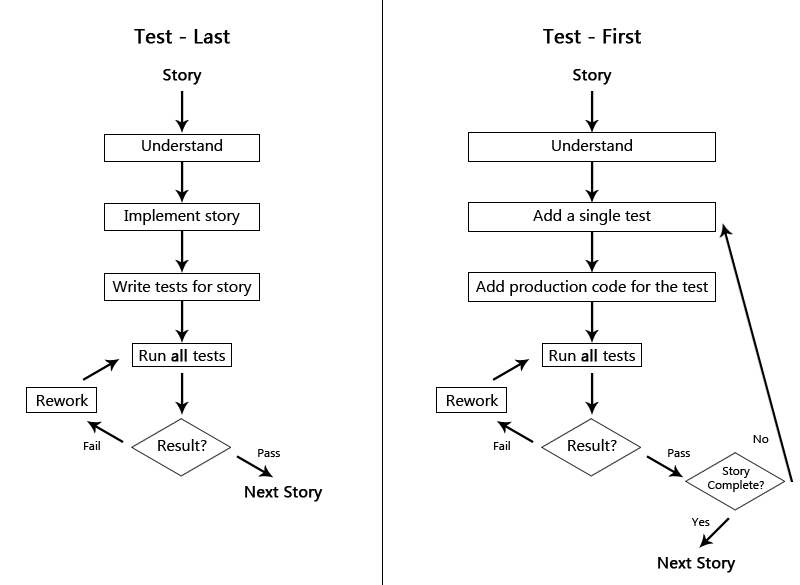
\includegraphics[scale=1]{tdd.png} 
% use appendices with more than one appendix
% then use \section to start each appendix
% you must declare a \section before using any
% \subsection or using \label (\appendices by itself
% starts a section numbered zero.)
%


%\appendices
%\ection{Proof of the First Zonklar Equation}
%Appendix one text goes here.

% you can choose not to have a title for an appendix
% if you want by leaving the argument blank
%\ection{}
%Appendix two text goes here.



% Can use something like this to put references on a page
% by themselves when using endfloat and the captionsoff option.
\ifCLASSOPTIONcaptionsoff
  \newpage
\fi



% trigger a \newpage just before the given reference
% number - used to balance the columns on the last page
% adjust value as needed - may need to be readjusted if
% the document is modified later
%\IEEEtriggeratref{8}
% The "triggered" command can be changed if desired:
%\IEEEtriggercmd{\enlargethispage{-5in}}

% references section

% can use a bibliography generated by BibTeX as a .bbl file
% BibTeX documentation can be easily obtained at:
% http://www.ctan.org/tex-archive/biblio/bibtex/contrib/doc/
% The IEEEtran BibTeX style support page is at:
% http://www.michaelshell.org/tex/ieeetran/bibtex/
%\bibliographystyle{IEEEtran}
% argument is your BibTeX string definitions and bibliography database(s)
%\bibliography{IEEEabrv,../bib/paper}
%
% <OR> manually copy in the resultant .bbl file
% set second argument of \begin to the number of references
% (used to reserve space for the reference number labels box)
\begin{thebibliography}{1}
\label{bibliography}

\bibitem{IEEEhowto:kopka} % Add referenses in the same way as this one, and call them by ~\cite{biblabel}
H.~Kopka and P.~W. Daly, \emph{A Guide to {\LaTeX}}, 3rd~ed.\hskip 1em plus
  0.5em minus 0.4em\relax Harlow, England: Addison-Wesley, 1999.

\bibitem{mullerandhagner}
M.~M\"{u}ller and O.~Hagner, \emph{Experiment about Test-first programming}, Volume: 149\hskip 1em plus
  0.5em minus 0.4em\relax Karlsruhe Univ., Germany, Comput. Sci. Dept., 2002. 

\bibitem{georgeandwilliams}
M.~M\"{u}ller and O.~Hagner, \emph{A structured experiment of test-driven development}, Volume: 149\hskip 1em plus
  0.5em minus 0.4em\relax Karlsruhe Univ., Germany, Comput. Sci. Dept., 2002. 
 
\bibitem{erdogmus}
Hakan Erdogmus, \emph{On the Effectiveness of Test-first Approach to Programming}\hskip 1em plus
  0.5em minus 0.4emBeck, K., Test Driven Development -- by Example. Boston: 
Addison Wesley, 2003.\relax NRC Institute for Information Technology; National Research Council Canada, 2005
 
\bibitem{janzen}
David Scott Janzen, \emph{An Empirical Evaluation of the Impact of Test-Driven Development on Software Quality.}\hskip 1em plus
  0.5em minus 0.4em\relax M.S., Computer Science, University of Kansas, 1993


\bibitem{microsoftibm}
Nachiappan Nagappan, E. Michael Maximilien et. al, \emph{Realizing quality improvement through test driven development: results and experiences of four industrial teams}\hskip 1em plus
  0.5em minus 0.4em\relax Springer Science + Business Media, LLC, 2008

\bibitem{sciencedirect}
\url{http://www.sciencedirect.com/science?_ob=MiamiImageURL&_cid=271539&_user=745831&_pii=S0950584903002040&_check=y&_origin=article&_zone=toolbar&_coverDate=15-Apr-2004&view=c&originContentFamily=serial&wchp=dGLbVlB-zSkWz&md5=16ebc0c991d5a69b0aef824fc619a012/1-s2.0-S0950584903002040-main.pdf}
 
 \bibitem{janzen2}
M.~M\"{u}ller and O.~Hagner, \emph{Test-driven development concepts, taxonomy, and future direction}, Volume: 149\hskip 1em plus
  0.5em minus 0.4em\relax Karlsruhe Univ., Germany, Comput. Sci. Dept., 2002.
  
  \bibitem{beckXP}
  Beck, K., Extreme Programming Explained:  Embrace Change. Reading, Massachusetts: Addison-Wesley, 2000.
  
  \bibitem{beckTestDriven}
Beck, K., Test Driven Development -- by Example. Boston: Addison Wesley, 2003.

  \bibitem{MSNET}
  Newkirk, JW and Vorontsov, AA. Test-Driven Development in Microsoft .NET, Microsoft Press, 2004.
  
  \bibitem{NASA}
  Larman, G. and V. R. Basili (2003). "Iterative and Incremental Development: A Brief History." IEEE Computer 36(6): 47 - 56.
  
  \bibitem{tddInvest}
  B. George and L. Williams, “An Initial Investigation of Test Driven Development in Industry,” Proc. ACM Symp. Applied Computing, 2003.
 

\bibitem{tddroi}
M.~M\"{u}ller and F.~Padberg, \emph{ About the Return on Investment of Test-Driven Development}
  EDSER-5 $5^{th}$ International Workshop on Economic-Driven Software Engineering Research, Portland, Oregon, May 3-11, 2003.


\bibitem{helloworld}
Brett L. Schuschert, \emph{Tdd.HelloWorld.Cpp} \hskip 1 em plus
  0.5em minus 0.4em\relax \url{http://schuschert.wikispaces.com/Tdd.HelloWorld.Cpp}, 2012-02-21.
  
 \bibitem{Chung}
Chung, L. (2009). Conceptual Modeling: Foundations and Applications On Non-Functional Requirements in Software Engineering. Conceptual
 Modeling: Foundations and Applications: Essays in Honor of John Mylopoulos, 5600, 363-379.doi:10.1007/978-3-642-02463-4\_19
 
 \bibitem{Galin}
 Galin, D. (2004). Software quality assurance. Harlow, England: Pearson Education Limited.
 
 \bibitem{ISO1061}
 IEEE Standard 1061-1992 Standard for a Software Quality Metrics Methodology. Institute
of Electrical and Electronics Engineers, New York (1992) 

\bibitem{cisq}
 \url{(http://www.it-cisq.org/cisqwiki/images/8/87/CISQ_2009_Executive_Forums_Report.pdf)}

 \bibitem{Pressman}    
 Pressman, Scott (2005), Software Engineering: A Practitioner's Approach (Sixth, International ed.), McGraw-Hill Education Pressman, p. 388
       
 \bibitem{ISO9126}
ISO International Organization for Standardization. (2003). ISO: Software engineering - product quality = Génie du logiciel - qualité des produits. Geneva: ISO.

\end{thebibliography}



% biography section
% 
% If you have an EPS/PDF photo (graphicx package needed) extra braces are
% needed around the contents of the optional argument to biography to prevent
% the LaTeX parser from getting confused when it sees the complicated
% \includegraphics command within an optional argument. (You could create
% your own custom macro containing the \includegraphics command to make things
% simpler here.)
%\begin{biography}[{\includegraphics[width=1in,height=1.25in,clip,keepaspectratio]{mshell}}]{Michael Shell}
% or if you just want to reserve a space for a photo:

%\begin{IEEEbiography}{Michael Shell}
%Biography text here.
%\end{IEEEbiography}
%
%% if you will not have a photo at all:
%\begin{IEEEbiographynophoto}{John Doe}
%Biography text here.
%\end{IEEEbiographynophoto}
%
%% insert where needed to balance the two columns on the last page with
%% biographies
%%\newpage
%
%\begin{IEEEbiographynophoto}{Jane Doe}
%Biography text here.
%\end{IEEEbiographynophoto}

% You can push biographies down or up by placing
% a \vfill before or after them. The appropriate
% use of \vfill depends on what kind of text is
% on the last page and whether or not the columns
% are being equalized.

%\vfill

% Can be used to pull up biographies so that the bottom of the last one
% is flush with the other column.
%\enlargethispage{-5in}



% that's all folks
\end{document}


